\PassOptionsToPackage{unicode=true}{hyperref} % options for packages loaded elsewhere
\PassOptionsToPackage{hyphens}{url}
%
\documentclass[]{article}
\usepackage{lmodern}
\usepackage{amssymb,amsmath}
\usepackage{ifxetex,ifluatex}
\usepackage{fixltx2e} % provides \textsubscript
\ifnum 0\ifxetex 1\fi\ifluatex 1\fi=0 % if pdftex
  \usepackage[T1]{fontenc}
  \usepackage[utf8]{inputenc}
  \usepackage{textcomp} % provides euro and other symbols
\else % if luatex or xelatex
  \usepackage{unicode-math}
  \defaultfontfeatures{Ligatures=TeX,Scale=MatchLowercase}
\fi
% use upquote if available, for straight quotes in verbatim environments
\IfFileExists{upquote.sty}{\usepackage{upquote}}{}
% use microtype if available
\IfFileExists{microtype.sty}{%
\usepackage[]{microtype}
\UseMicrotypeSet[protrusion]{basicmath} % disable protrusion for tt fonts
}{}
\IfFileExists{parskip.sty}{%
\usepackage{parskip}
}{% else
\setlength{\parindent}{0pt}
\setlength{\parskip}{6pt plus 2pt minus 1pt}
}
\usepackage{hyperref}
\hypersetup{
            pdfborder={0 0 0},
            breaklinks=true}
\urlstyle{same}  % don't use monospace font for urls
\usepackage[left=2cm,right=2cm,top=1cm,bottom=2cm]{geometry}
\usepackage{color}
\usepackage{fancyvrb}
\newcommand{\VerbBar}{|}
\newcommand{\VERB}{\Verb[commandchars=\\\{\}]}
\DefineVerbatimEnvironment{Highlighting}{Verbatim}{commandchars=\\\{\}}
% Add ',fontsize=\small' for more characters per line
\newenvironment{Shaded}{}{}
\newcommand{\AlertTok}[1]{\textcolor[rgb]{1.00,0.00,0.00}{\textbf{#1}}}
\newcommand{\AnnotationTok}[1]{\textcolor[rgb]{0.38,0.63,0.69}{\textbf{\textit{#1}}}}
\newcommand{\AttributeTok}[1]{\textcolor[rgb]{0.49,0.56,0.16}{#1}}
\newcommand{\BaseNTok}[1]{\textcolor[rgb]{0.25,0.63,0.44}{#1}}
\newcommand{\BuiltInTok}[1]{#1}
\newcommand{\CharTok}[1]{\textcolor[rgb]{0.25,0.44,0.63}{#1}}
\newcommand{\CommentTok}[1]{\textcolor[rgb]{0.38,0.63,0.69}{\textit{#1}}}
\newcommand{\CommentVarTok}[1]{\textcolor[rgb]{0.38,0.63,0.69}{\textbf{\textit{#1}}}}
\newcommand{\ConstantTok}[1]{\textcolor[rgb]{0.53,0.00,0.00}{#1}}
\newcommand{\ControlFlowTok}[1]{\textcolor[rgb]{0.00,0.44,0.13}{\textbf{#1}}}
\newcommand{\DataTypeTok}[1]{\textcolor[rgb]{0.56,0.13,0.00}{#1}}
\newcommand{\DecValTok}[1]{\textcolor[rgb]{0.25,0.63,0.44}{#1}}
\newcommand{\DocumentationTok}[1]{\textcolor[rgb]{0.73,0.13,0.13}{\textit{#1}}}
\newcommand{\ErrorTok}[1]{\textcolor[rgb]{1.00,0.00,0.00}{\textbf{#1}}}
\newcommand{\ExtensionTok}[1]{#1}
\newcommand{\FloatTok}[1]{\textcolor[rgb]{0.25,0.63,0.44}{#1}}
\newcommand{\FunctionTok}[1]{\textcolor[rgb]{0.02,0.16,0.49}{#1}}
\newcommand{\ImportTok}[1]{#1}
\newcommand{\InformationTok}[1]{\textcolor[rgb]{0.38,0.63,0.69}{\textbf{\textit{#1}}}}
\newcommand{\KeywordTok}[1]{\textcolor[rgb]{0.00,0.44,0.13}{\textbf{#1}}}
\newcommand{\NormalTok}[1]{#1}
\newcommand{\OperatorTok}[1]{\textcolor[rgb]{0.40,0.40,0.40}{#1}}
\newcommand{\OtherTok}[1]{\textcolor[rgb]{0.00,0.44,0.13}{#1}}
\newcommand{\PreprocessorTok}[1]{\textcolor[rgb]{0.74,0.48,0.00}{#1}}
\newcommand{\RegionMarkerTok}[1]{#1}
\newcommand{\SpecialCharTok}[1]{\textcolor[rgb]{0.25,0.44,0.63}{#1}}
\newcommand{\SpecialStringTok}[1]{\textcolor[rgb]{0.73,0.40,0.53}{#1}}
\newcommand{\StringTok}[1]{\textcolor[rgb]{0.25,0.44,0.63}{#1}}
\newcommand{\VariableTok}[1]{\textcolor[rgb]{0.10,0.09,0.49}{#1}}
\newcommand{\VerbatimStringTok}[1]{\textcolor[rgb]{0.25,0.44,0.63}{#1}}
\newcommand{\WarningTok}[1]{\textcolor[rgb]{0.38,0.63,0.69}{\textbf{\textit{#1}}}}
\usepackage{graphicx,grffile}
\makeatletter
\def\maxwidth{\ifdim\Gin@nat@width>\linewidth\linewidth\else\Gin@nat@width\fi}
\def\maxheight{\ifdim\Gin@nat@height>\textheight\textheight\else\Gin@nat@height\fi}
\makeatother
% Scale images if necessary, so that they will not overflow the page
% margins by default, and it is still possible to overwrite the defaults
% using explicit options in \includegraphics[width, height, ...]{}
\setkeys{Gin}{width=\maxwidth,height=\maxheight,keepaspectratio}
\setlength{\emergencystretch}{3em}  % prevent overfull lines
\providecommand{\tightlist}{%
  \setlength{\itemsep}{0pt}\setlength{\parskip}{0pt}}
\setcounter{secnumdepth}{0}
% Redefines (sub)paragraphs to behave more like sections
\ifx\paragraph\undefined\else
\let\oldparagraph\paragraph
\renewcommand{\paragraph}[1]{\oldparagraph{#1}\mbox{}}
\fi
\ifx\subparagraph\undefined\else
\let\oldsubparagraph\subparagraph
\renewcommand{\subparagraph}[1]{\oldsubparagraph{#1}\mbox{}}
\fi

% set default figure placement to htbp
\makeatletter
\def\fps@figure{htbp}
\makeatother


\date{}

\begin{document}

\hypertarget{progetto-concettuale}{%
\subsection{\texorpdfstring{\texttt{Progetto\ concettuale}}{Progetto concettuale}}\label{progetto-concettuale}}

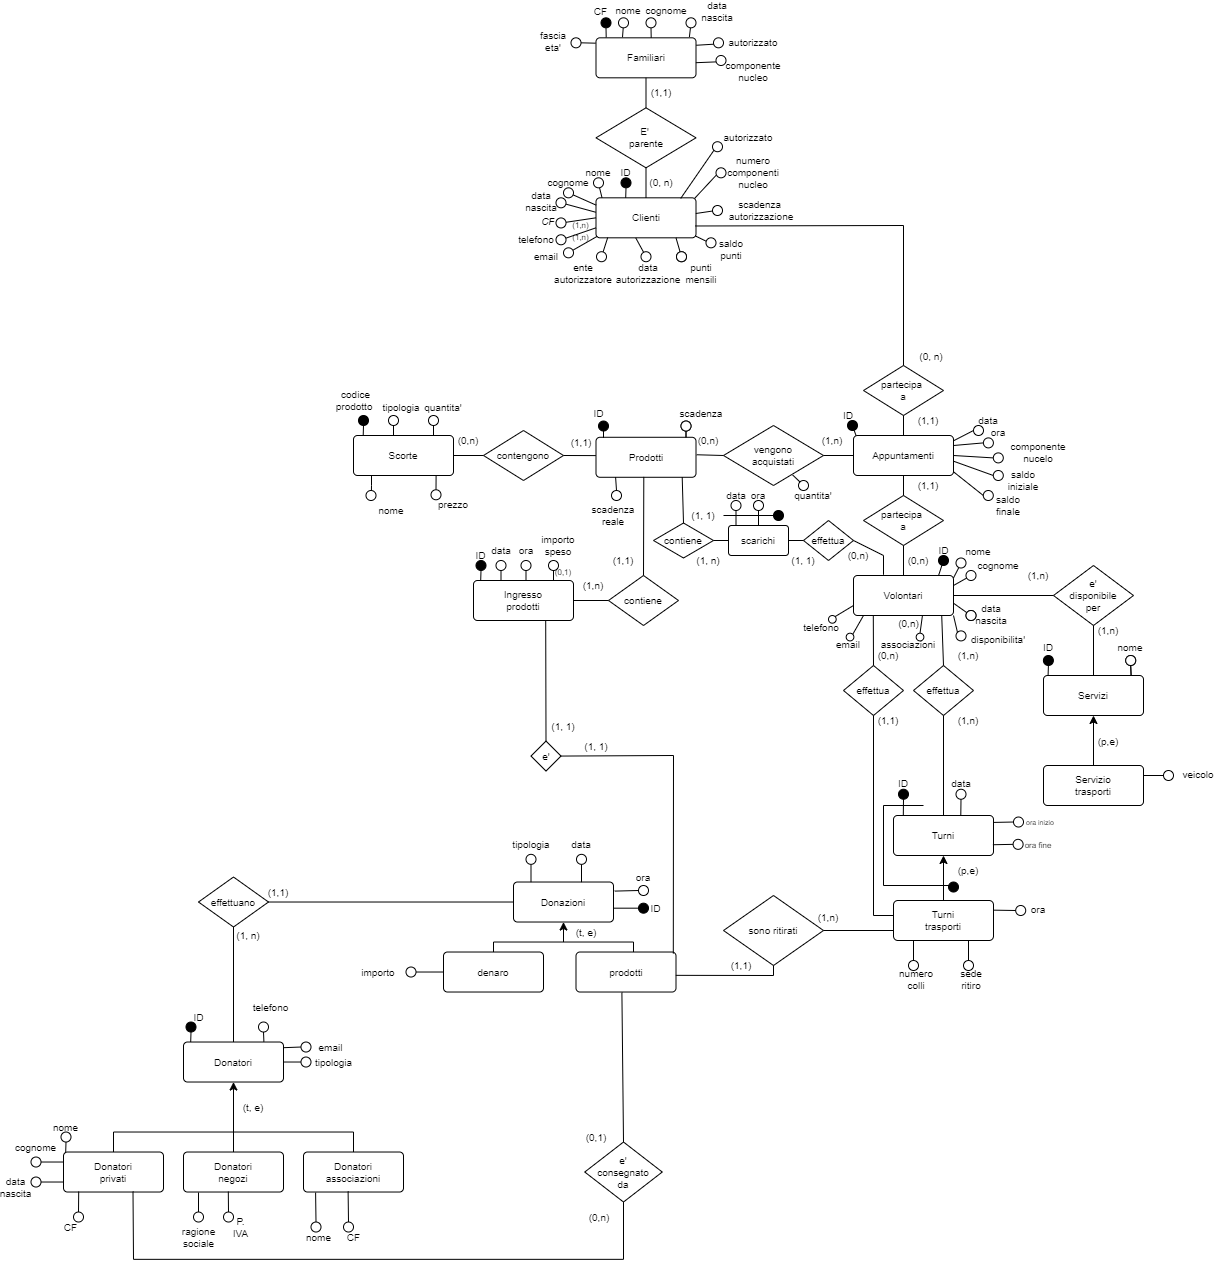
\includegraphics{social_market_v2.drawio.png}

\newpage

\begin{figure}
\centering
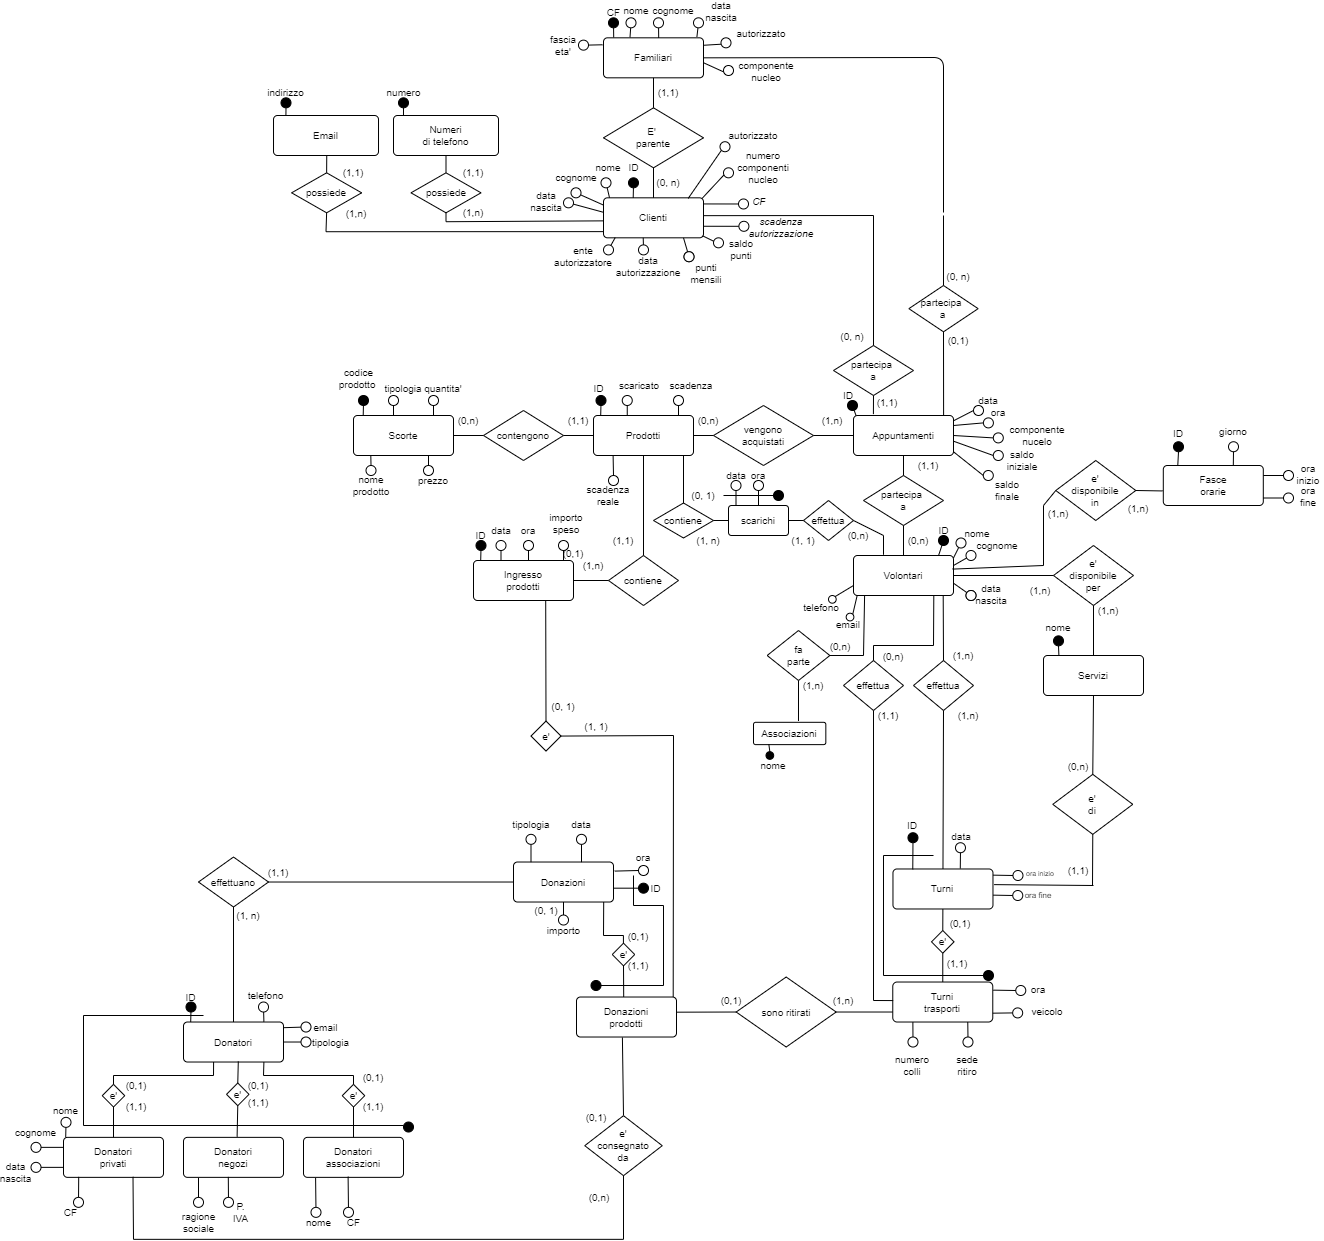
\includegraphics{social_market_v2_ristrutturato.drawio.png}
\caption{Diagramma ER ristrutturato}
\end{figure}

\newpage

\hypertarget{requisiti-informativi}{%
\subsubsection{\texorpdfstring{\texttt{requisiti\ informativi}}{requisiti informativi}}\label{requisiti-informativi}}

Le specifiche richiedono una base di dati in grado di eseguire
operazioni abbastanza diverse tra loro, come:

\begin{itemize}
\tightlist
\item
  programmazione turni dei volontari
\item
  inventario dei prodotti (e relative operazioni)
\item
  ricezione dei clienti su appuntamento e relativo acquisto dei prodotti
\item
  ricezione donazioni
\end{itemize}

Ovviamente, tutte queste operazioni non sono indipendenti tra di loro
(esempio: i volontari oltre ad essere coloro che ritirano le donazioni
sono anche quelli che accolgono i clienti agli appuntamenti), quindi e'
necessario pensare bene alle caratteristiche che la nostra base di dati
debba avere.

Per molte tabelle abbiamo specificato un \texttt{ID} come chiave
primaria (nonstante la presenza di altre chiavi candidate) piu' che
altro per una questione di efficienza, per esempio una chiave candidata
di \texttt{Cliente} potrebbe essere il codice fiscale, pero' in
un'ipotetico utilizzo dove bisogna ricercare un cliente specifico la
ricerca avviene piu' velocemente confrontato numeri interi anziche'
stringhe.

\hypertarget{implementazione}{%
\subsection{\texorpdfstring{\texttt{Implementazione}}{Implementazione}}\label{implementazione}}

\hypertarget{clienti}{%
\paragraph{\texorpdfstring{\texttt{Clienti}}{Clienti}}\label{clienti}}

per i clienti vengono memorizzati rispettivamente:

\begin{itemize}
\tightlist
\item
  \textbf{ID}
\item
  nome
\item
  cognome
\item
  data di nascita
\item
  codice fiscale
\item
  numero/i di telefono
\item
  email
\item
  ente che gli ha concesso l'autorizzazione
\item
  data dell'autorizzazione
\item
  scadenza dell'autorizzazione (default 6 mesi dalla data di
  autorizzazione)
\item
  punti mensili
\item
  saldo punti
\item
  numero dei componenti del nucleo familiare
\item
  se e' autorizzato o meno a spendere i punti
\end{itemize}

l'\texttt{ID} viene utilizzato per identificare il singolo cliente per i
motivi specificati sopra, inoltre abbiamo deciso di salvare i dati
anagrafici dei familiari del cliente in un'altra entita', in modo che un
cliente possa avere piu' familiari. Abbiamo salvato il flag
\texttt{\textquotesingle{}autorizzato\textquotesingle{}} sia nei
familiari che nei clienti perche' reputiamo che un possibile che ad un
cliente venga tolta l'autorizzazione a spendere i punti ma alla sua
famiglia no.

\hypertarget{vincoli-dintegrita}{%
\subparagraph{\texorpdfstring{\texttt{vincoli\ d\textquotesingle{}integrita\textquotesingle{}}}{vincoli d'integrita'}}\label{vincoli-dintegrita}}

\begin{itemize}
\tightlist
\item
  \(Clienti(ID)\) e' chiave primaria di \texttt{Clienti}
\item
  \(Clienti(CF)\) e' \texttt{UNIQUE}
\item
  \(Clienti(scadenza\_autorizzazione)\) sara' calcolata con un trigger
  su insert inserendo in quel campo data\_autorizzazione + 6 mesi
\item
  \(Familiari(CF)\) e' chiave primaria di \texttt{Familiari}
\item
  \(Familiari(telefono)\) e' \texttt{opzionale} e \texttt{UNIQUE}
\item
  \(Familiari(email)\) e' \texttt{opzionale} e \texttt{UNIQUE}
\item
  \(Familiari(ID\_cliente^{cliente})\) ha \texttt{ON\ DELETE\ CASCADE}
  perche' e' sensato che, se un cliente viene disinserito, anche tutta
  la sua famiglia non possa piu' comprare al market. E
  \texttt{ON\ UPDATE\ CASCADE}
\end{itemize}

\hypertarget{volontari}{%
\paragraph{\texorpdfstring{\texttt{Volontari}}{Volontari}}\label{volontari}}

Per ogni volontario memorizziamo:

\begin{itemize}
\tightlist
\item
  \textbf{ID}
\item
  nome
\item
  cognome
\item
  data di nascita
\item
  numero di telefono
\item
  email
\item
  eventuali associazioni a cui e' collegato
\end{itemize}

Per i volontari abbiamo pensato di ammetere un solo numero di telefono e
una sola email, perche' a differenza dei clienti in questo caso questi
contatti devono essere univoci per ogni volontario, mentre per i clienti
e' possibile che ogni familiare dia per esempio una mail differente a
cui essere contattato.

\hypertarget{vincoli-dintegrita-1}{%
\subparagraph{\texorpdfstring{\texttt{vincoli\ d\textquotesingle{}integrita\textquotesingle{}}}{vincoli d'integrita'}}\label{vincoli-dintegrita-1}}

\begin{itemize}
\tightlist
\item
  \(ID\) e' \texttt{chiave\ primaria}
\item
  \(email\) e' \texttt{UNIQUE}
\item
  \(telefono\) e' \texttt{UNIQUE}
\item
  Puo' non essere collegato a nessuna associazione
\end{itemize}

\hypertarget{inventario-prodotti}{%
\paragraph{\texorpdfstring{\texttt{Inventario\ prodotti}}{Inventario prodotti}}\label{inventario-prodotti}}

Per implementare lo stoccaggio dei prodotti abbiamo pensto a diverse
alternative, ma in base a diverse considerazioni sul carico di lavoro
siamo arrivati alla seguente implementazione:

\begin{itemize}
\tightlist
\item
  \textbf{ID}
\item
  nome
\item
  prezzo (in punti)
\item
  scadenza
\item
  scadenza ``reale'' (ovvero la data oltre la data di scadenza in cui
  non e' piu' possibile utilizzare il prodotto)
\end{itemize}

In questo caso, l'\texttt{ID} e' riferito al singolo prodotto, quindi se
come ingresso prodotti avessimo 50 confezioni verrebbero materialmente
inserite 50 tuple con ID diverso nell'entita' \texttt{Prodotti}. Siccome
pero' e' possibile che queste 50 confezioni di shampoo abbiano tutte una
data di scadenza diversa, in questo modo non e' possibile memorizzare la
quantita' in magazzino di uno specifico shampoo. Per risolvere questo
problema abbiamo inserito una nuova entita'
\texttt{\textquotesingle{}Scorte\textquotesingle{}} che memorizza un
\texttt{codice\ per\ ogni\ marca\ di\ prodotto} (es. 6298
-\textgreater{} tipologia: `Tonno', Marca: `Rio Mare'), insieme alle
relative quantita' disponibili.

Vengono memorizzati inoltre tutti gli
\textbf{\texttt{ingressi\ di\ prodotti}}, con la relativa data e ora. E'
ovviamente possibile recuperare a quale ingresso prodotti corrisponde un
determinato prodotto e se e' stato acquistato o donato.

\hypertarget{vincoli-dintegrita-2}{%
\subparagraph{\texorpdfstring{\texttt{vincoli\ d\textquotesingle{}integrita\textquotesingle{}}}{vincoli d'integrita'}}\label{vincoli-dintegrita-2}}

\begin{itemize}
\tightlist
\item
  \(Prodotti(ID)\) e' \texttt{chiave\ primaria} di \(Prodotti\)
\item
  \(Scorte(codice\_prodotto)\) e' \texttt{chiave\ primaria} di
  \(Scorte\)
\item
  \(Ingresso\_prodotti(ID)\) e' \texttt{chiave\ primaria} di
  \(Ingresso\ prodotti\)
\item
  \(Ingresso\_prodotti(data), Ingresso\_prodotti(ora)\) sono
  \texttt{UNIQUE} insieme
\item
  \(Ingresso\_prodotti(ID), Acquisto(importo\_speso)\) sono insieme
  \texttt{chiave\ primaria} di \(Acquisto\) (quindi decidiamo di tenere
  la chiave primaria di \(Ingresso\ prodotti\) in \(Acquisto\))
\item
  \(Ingresso\_prodotti(data), Ingresso\_prodotti(ora)\) sono
  \texttt{UNIQUE} insieme
\item
  \(Prodotti(codice\_prodotto^{Scorte})\) \texttt{ON\ DELETE\ CASCADE} e
  \texttt{ON\ UPDATE\ CASCADE}
\item
  \(Prodotti(ID\_ingresso^{Ingresso\_prodotti})\)
  \texttt{ON\ DELETE\ CASCADE} e \texttt{ON\ UPDATE\ CASCADE}
\item
  \(Prodotti(data\_scarico^{Scarichi})\) ha
  \texttt{ON\ DELETE\ SET\ NULL} e \texttt{ON\ UPDATE\ CASCADE}
\item
  \(Prodotti(ora\_scarico^{Scarichi})\) ha
  \texttt{ON\ DELETE\ SET\ NULL} e \texttt{ON\ UPDATE\ CASCADE}
\end{itemize}

\hypertarget{appuntamenti}{%
\paragraph{\texorpdfstring{\texttt{Appuntamenti}}{Appuntamenti}}\label{appuntamenti}}

Ogni appuntamento viene memorizzato salvando la
\texttt{data,\ l\textquotesingle{}ora,\ il\ componente\ del\ nucleo\ familiare\ che\ vi\ prende\ parte,\ il\ saldo\ punti\ prima\ e\ dopo\ gli\ acquisti}.
Utilizziamo anche in questo caso un \texttt{ID} come chiave perche' e'
un poco piu' efficiente e comodo rispetto ad usare la data e l'ora
insieme. Ogni appuntamento dura 15 minuti e si distanziano l'un l'altro
di 5 minuti. Per implementare questa funzione usiamo un trigger su
insert, che controlla che l'appuntamento che si sta inserendo non
``esuberi'' all'interno di un altro appuntamento gia' fissato (quindi se
la data e l'ora \(\pm\) 20 minuti non siano gia' presenti nella
tabella).

\hypertarget{vincoli-dintegrita-3}{%
\subparagraph{\texorpdfstring{\texttt{vincoli\ d\textquotesingle{}integrita\textquotesingle{}}}{vincoli d'integrita'}}\label{vincoli-dintegrita-3}}

\begin{itemize}
\tightlist
\item
  \(ID\) e' \texttt{chiave\ primaria}
\item
  \(data,\ ora\) sono \texttt{UNIQUE} insieme
\item
  \(saldo\ iniziale\) e' settato tramite un trigger su insert e prende
  il saldo iniziale del cliente
\item
  \(ID\_cliente^{clienti}\) ha \texttt{ON\ DELETE\ NO\ ACTION} e
  \texttt{ON\ UPDATE\ CASCADE}
\item
  \(ID\_volontario^{volontari}\) ha \texttt{ON\ DELETE\ NO\ ACTION} e
  \texttt{ON\ UPDATE\ CASCADE}
\end{itemize}

\hypertarget{donazioni}{%
\paragraph{\texorpdfstring{\texttt{Donazioni}}{Donazioni}}\label{donazioni}}

Le donazioni possono essere in denaro o in prodotti e possono essere
effettuati da diversi \texttt{donatori} (privati, associazioni oppure
negozi). Abbiamo implementato il tutto facendo due macro categorie
(generalizzazioni) \texttt{Donazioni} e \texttt{Donatori}, a cui
corrispondono rispettivamente \texttt{privati}, \texttt{negozi},
\texttt{associazioni} e \texttt{denaro}, \texttt{prodotti}. Per ogni
donatore vengono memorizzati i vari recapiti (telefono, email) anche in
questo caso univoci e la tipologia del donatore (appunto privato,
negozio o associazione)

\hypertarget{vincoli-dintegrita-4}{%
\subparagraph{\texorpdfstring{\texttt{vincoli\ d\textquotesingle{}integrita\textquotesingle{}}}{vincoli d'integrita'}}\label{vincoli-dintegrita-4}}

\begin{itemize}
\tightlist
\item
  \(Donazioni(ID)\) e' \texttt{chiave\ primaria} di \(Donazioni\)
\item
  \(Donazioni(ID)\) e' \texttt{chiave\ primaria} di
  \(Donazioni \to Prodotti\)
\item
  \(Donazioni(ID)\) e' \texttt{chiave\ primaria} di
  \(Donazioni \to Denaro\)
\item
  \(Donatori(ID)\) e' \texttt{chiave\ primaria} di \(Donatori\)
\item
  \(Donatori(ID)\) e' \texttt{chiave\ primaria} di
  \(Donatori \to Privati\)
\item
  \(Donatori(ID)\) e' \texttt{chiave\ primaria} di
  \(Donatori \to Negozi\)
\item
  \(Donatori(ID)\) e' \texttt{chiave\ primaria} di
  \(Donatori \to Associazioni\)
\item
  \(Donazioni(data), Donazioni(ora)\) sono \texttt{UNIQUE} insieme
\item
  \(Donatori(telefono)\) e' \texttt{UNIQUE}
\item
  \(Donatori(email)\) e' \texttt{UNIQUE}
\item
  \((Donatori \to Privati)(CF)\) e' \texttt{UNIQUE}
\item
  \((Donatori \to Negozi)(P.\ IVA)\) e' \texttt{UNIQUE}
\item
  \((Donatori \to Negozi)(ragione\_sociale)\) e' \texttt{UNIQUE}
\item
  \((Donatori \to Associazioni)(CF)\) e' \texttt{UNIQUE}
\item
  \((Donatori \to Associazioni)(nome)\) e' \texttt{UNIQUE}
\item
  \((Donazioni \to Prodotti)(ID\_consegnatario\_privato^{Donatori \to Privati})\)
  puo' essere \texttt{NULL}
\item
  \((Donazioni \to Prodotti)(ID\_consegnatario\_privato^{Donatori \to Privati})\)
  ha \texttt{ON\ DELETE\ NO\ ACTION} e \texttt{ON\ UPDATE\ CASCADE}
\item
  \((Donazioni \to Prodotti)(ID\_ingresso\_prodotti^{Ingresso\_prodotti})\)
  ha \texttt{ON\ DELETE\ CASCADE} e \texttt{ON\ UPDATE\ CASCADE}
\end{itemize}

\hypertarget{turni}{%
\subsubsection{\texorpdfstring{\texttt{Turni}}{Turni}}\label{turni}}

I turni vengono memorizzati nel DB con la relativa \texttt{data},
\texttt{ora\ di\ inizio} e \texttt{ora\ di\ fine} turno. C'e' inoltre
una specializzazione di un normale turno che e' il turno relativo a un
trasporto merci, di cui salviamo anche il \texttt{numero\ di\ colli}
trasportati e la \texttt{sede\ del\ ritiro}, oltre che la
\texttt{data\ e\ ora}.

\hypertarget{vincoli-dintegrita-5}{%
\paragraph{\texorpdfstring{\texttt{vincoli\ d\textquotesingle{}integrita\textquotesingle{}}}{vincoli d'integrita'}}\label{vincoli-dintegrita-5}}

\begin{itemize}
\tightlist
\item
  \(Turni(data), Turni(ora\_inzio), Turni(ora\_fine)\) sono insieme
  \texttt{chiave\ primaria} di \(Turni\)
\item
  \(Turni(data), (Turni \to Trasporti)(ora)\) e'
  \texttt{chiave\ primaria} di \(Turni \to Trasporti\)
\end{itemize}

\hypertarget{servizi-dei-volontari}{%
\subsubsection{\texorpdfstring{\texttt{Servizi\ dei\ volontari}}{Servizi dei volontari}}\label{servizi-dei-volontari}}

Ogni volontario puo' essere disponibile in determianti giorni e orari
per determinati servizi (anche piu' di uno), per ogni servizio si
memorizza un \texttt{ID} e il \texttt{nome} del servizio (es. Stoccaggio
merci magazzino), in particolare un servizio piu' specifico e' il
trasporto, di cui si memorizza anche il tipo di \texttt{veicolo}.

\hypertarget{vincoli-dintegrita-6}{%
\paragraph{\texorpdfstring{\texttt{vincoli\ d\textquotesingle{}integrita\textquotesingle{}}}{vincoli d'integrita'}}\label{vincoli-dintegrita-6}}

\begin{itemize}
\tightlist
\item
  \(Servizi(ID)\) e' \texttt{chiave\ primaria} di \(Servizi\)
\item
  \(Servizi(ID)\) e' \texttt{chiave\ primaria} di
  \(Servizi \to Trasporti\)
\end{itemize}

\hypertarget{scarico-prodotti-scaduti}{%
\subsubsection{\texorpdfstring{\texttt{Scarico\ prodotti\ scaduti}}{Scarico prodotti scaduti}}\label{scarico-prodotti-scaduti}}

Abbiamo implementato lo scarico dei prdotti tramite un'entita' in cui
vengono salvate la data e l'ora dello scarico. In questo caso non
conviene un \texttt{ID}, perche' poi in fase di implementazione avremo
due colonne aggiuntive nella tabella prodotti che saranno
\texttt{data\_scarico} e \texttt{ora\_scarico}, direttamente accessibili
senza la necessita' di fare un join per poterle recuperare.

\hypertarget{vincoli-dintegrita-7}{%
\paragraph{\texorpdfstring{\texttt{vincoli\ d\textquotesingle{}integrita\textquotesingle{}}}{vincoli d'integrita'}}\label{vincoli-dintegrita-7}}

\begin{itemize}
\tightlist
\item
  \(Scarichi(data), Scarichi(ora)\) sono insieme
  \texttt{chiave\ primaria} di \(Scarichi\)
\item
  \(Scarichi(ID\_volontario^{Volontari})\) ha
  \texttt{ON\ DELETE\ CASCADE} e \texttt{ON\ UPDATE\ CASCADE}
\end{itemize}

\hypertarget{carico-di-lavoro}{%
\subsection{\texorpdfstring{\texttt{carico\ di\ lavoro}}{carico di lavoro}}\label{carico-di-lavoro}}

Per effettuare tutte le operazioni al meglio, e' necessario stimare un
carico di lavoro (quali operazioni verranno fatte piu' spesso, il volume
dei dati nel tempo\ldots{}).

Essendo un social market, ci si aspetta che abbia (sfortunatamente)
abbastanza clienti ma non nell'ordine delle decine di milioni, per
esempio. Sapendo che la popolazione italiana e' di circa \(60,262,778\)
e che le persone in poverta' assoluta sono circa \(5,600,000\) nel 2022
(dati ISTAT), in percentuale siamo sul circa \(10,8\%\). Ora, prendendo
la popolazione per esempio di Genova nello stesso anno (\(568,999\)), il
\(10,8\%\) corrisponde a circa \(61,451.892\), approssimato diventa
\(61,452\). In ogni caso siamo sulle
\texttt{decine/centiaia\ di\ migliaia\ (per\ le\ citta\textquotesingle{}\ piu\textquotesingle{}\ popolose)\ di\ clienti}.
Occorre notare che per ogni cliente in media si avra' una famiglia al
seguito, quindi, supponendo che mediamente le famiglie siano formate da
\(4\) persone, si avra' qualche \texttt{centiaia\ di\ migliaia}
\(\cdot\) \texttt{4}, che nel caso delle citta' piu' popolose (es. Roma)
esubera il milione di circa \texttt{200k}. Quindi, nel caso peggiore, si
avranno \texttt{1.200.000} clienti tra clienti autorizzati e i loro
familiari.

Sapendo all'incirca quanti clienti si hanno, ci si potra' piu' o meno
orientare per capire di quanti prodotti il market avra' bisogno,
sicuramente piu' dei clienti. Quindi si suppone che, per quantita', i
prodotti saranno quelli con il maggior volume tra tutti gli altri dati,
seguiti dai clienti (e i loro familiari).

Si suppone che le operazioni svolte maggiormente saranno lo stoccaggio
dei prodotti in inventario (quindi inserimenti di prodotti e modifiche
delle quantita' nelle scorte), quindi bisogna cercare di non sprecare
memoria (per esempio con colonne a \texttt{null}) e bisogna ottimizzare
le operazioni in particolare su questi dati. Ovviamente anche le altre
operazioni (es. creazione turni) verranno fatte regolarmente, pero' non
avranno mai milioni di righe come per i clienti o i prodotti in
inventario.

\hypertarget{schema-logico}{%
\subsection{\texorpdfstring{\texttt{Schema\ logico}}{Schema logico}}\label{schema-logico}}

\textbf{Familiari}(\underline{CF}, nome, cognome, data\_nascita,
autorizzato, cliente\(^{clienti}\))

\textbf{Clienti}(\underline{ID}, nome, cognome, data\_nascita,
ente\_autorizzatore, data\_autorizzazione, punti\_mensili, saldo\_punti,
\emph{CF}, n\_componenti\_nucleo, autorizzato)

\textbf{Telefoni}(\underline{numero}, cliente\(^{clienti}\))

\textbf{Email}(\underline{indirizzo}, cliente\(^{clienti}\))

\textbf{Appuntamenti}(\underline{ID}, data, ora, componente\_nucleo,
saldo\_iniziale, saldo\_finale, cliente\(^{clienti}\),
volontario\(^{volontari}\))

\textbf{Prodotti}(\underline{ID}, nome, prezzo, scadenza,
scadenza\_reale, codice\_prodotto\(^{scorte}\),
ingresso\_prodotti\(^{ingresso\_prodotti}\),
data\_scarico\(^{scarichi}\), ora\_scarico\(^{scarichi}\))

\textbf{Scorte}(\underline{codice\_prodotto}, tipologia, marca,
quantita')

\textbf{Ingresso\_prodotti}(\underline{ID}, data, ora)

\textbf{Acquisto}(\underline{ID\_ingresso$^{ingresso\_prodotti}$},
importo\_speso)

\textbf{Volontari}(\underline{ID}, nome, cognome, data\_nascita,
\emph{telefono}, \emph{email})

\textbf{Associazioni}(\underline{nome})

\textbf{Servizi}(\underline{ID}, nome, veicolo\(_o\))

\textbf{Servizio\_trasporti}(\underline{ID\_servizio$^{servizi}$},
veicolo)

\textbf{Turni}(\underline{data, ora\_inizio, ora\_fine})

\textbf{Turno\_trasporti}(\underline{data$^{turni}$, ora},
numero\_colli, sede\_ritiro)

\textbf{Donazioni}(\underline{ID}, tipologia, data, ora,
donatore\(^{donatori}\))

\textbf{Donazioni\_denaro}(\underline{donazione$^{donazioni}$}, importo)

\textbf{Donazioni\_prodotti}(\underline{donazione$^{donazioni}$},
consegnatario\_privato\(^{donatori\_privati}_o\),
ingresso\_prodotti\(^{ingresso\_prodotti}\))

\textbf{Donatori}(\underline{ID}, \emph{telefono}, \emph{email},
tipologia)

\textbf{Donatori\_privati}(\underline{ID$^{donatori}$}, nome, cognome,
data\_nascita, \emph{CF})

\textbf{Donatori\_negozi}(\underline{ID$^{donatori}$}, ragione\_sociale,
\emph{p\_iva})

\textbf{Donatori\_associazioni}(\underline{ID$^{donatori}$}, nome,
\emph{CF})

\hypertarget{associazioni-nn}{%
\paragraph{\texorpdfstring{\texttt{associazioni\ (n,n)}}{associazioni (n,n)}}\label{associazioni-nn}}

\textbf{appuntamenti\_prodotti}(\underline{codice\_prodotto$^{scorte}$, appuntamento$^{appuntamenti}$},
quantita')

\textbf{volontari\_associazioni}(\underline{volontario$^{volontari}$, associazione$^{associazioni}$})

\textbf{volontari\_turni}(\underline{volontario$^{volontari}$, data\_turno$^{turni}$, ora\_inizio\_turno$^{turni}$, ora\_fine\_turno$^{turni}$})

\textbf{volontari\_servizi}(\underline{volontario$^{volontari}$, servizio$^{servizi}$},
finestra\_temporale)

\textbf{volontario\_prodotti\_donati}(\underline{volontario$^{volontari}$, *donazione*$^{donazioni}$})

\hypertarget{normalizzazione}{%
\subsection{\texorpdfstring{\texttt{Normalizzazione}}{Normalizzazione}}\label{normalizzazione}}

Per verificare la qualita' dello schema ER ristrutturato e' bene
controllare che rispetti la \texttt{forma\ normale\ di\ Boyce\ Codd} e,
nel caso non la rispettasse e non fosse possibile decomporre lo schema
in modo da fargliela rispettare, la \texttt{terza\ forma\ normale} (che
invece e' sempre possibile). Cominciamo elencando le dipendenze
funzionali

\begin{itemize}
\tightlist
\item
  Familiari(CF, nome, cognome, data\_nascita, cliente\(^{clienti}\))

  \begin{itemize}
  \tightlist
  \item
    \(CF \to nome, cognome, data\_nascita\)
  \item
    \(cliente^{clienti} \to CF\)
  \end{itemize}
\item
  Clienti

  \begin{itemize}
  \tightlist
  \item
    \(ID \to nome, cognome, data\_nascita, ente\_autorizzatore\),
    \(data\_autorizzazione, punti\_mensili, saldo\_punti, CF, autorizzato, n\_componenti\_nucleo\)
  \item
    \(CF \to nome, cognome, data\_nascita\)
  \end{itemize}
\item
  Appuntamenti

  \begin{itemize}
  \tightlist
  \item
    \(ID \to data, ora, componente\_nucleo, saldo\_iniziale, saldo\_finale\)
  \item
    \(data, ora \to ID, componente\_nucleo, saldo\_iniziale, saldo\_finale\)
  \end{itemize}
\item
  Prodotti

  \begin{itemize}
  \tightlist
  \item
    \(ID \to nome, prezzo, scadenza, scadenza\_reale\)
  \end{itemize}
\item
  Scorte

  \begin{itemize}
  \tightlist
  \item
    \(codice\_prodotto \to tipologia, quantita'\)
  \end{itemize}
\item
  Ingresso prodotti

  \begin{itemize}
  \tightlist
  \item
    \(ID \to data, ora\)
  \end{itemize}
\end{itemize}

\hypertarget{query}{%
\subsection{\texorpdfstring{\texttt{Query}}{Query}}\label{query}}

Tutti i prodotti acquistati durante l'ultimo appuntamento del cliente
con ID = 1

\begin{Shaded}
\begin{Highlighting}[]
\KeywordTok{SELECT} \OperatorTok{*} 
\KeywordTok{FROM}\NormalTok{ Prodotti}
\KeywordTok{JOIN}\NormalTok{ Appuntamenti_prodotti}
\KeywordTok{ON}\NormalTok{ Appuntamenti_prodotti.prodotto }\OperatorTok{=}\NormalTok{ prodotti.}\KeywordTok{ID}
\KeywordTok{JOIN}\NormalTok{ Appuntamenti}
\KeywordTok{ON}\NormalTok{ Appuntamenti_prodotti.appuntamento }\OperatorTok{=}\NormalTok{ Appuntamenti.}\KeywordTok{ID}
\KeywordTok{JOIN}\NormalTok{ Clienti}
\KeywordTok{ON}\NormalTok{ Appuntamenti.cliente }\OperatorTok{=}\NormalTok{ Clienti.}\KeywordTok{ID}
\KeywordTok{WHERE}\NormalTok{ Clienti.}\KeywordTok{ID} \OperatorTok{=} \DecValTok{1}
\end{Highlighting}
\end{Shaded}

\end{document}
